\documentclass[11pt]{article}
\usepackage[T1]{fontenc}
\usepackage{lmodern,amsmath,amssymb,microtype,geometry,xcolor,pdfpages,hyperref}
\geometry{margin=1.02in}
\definecolor{ink}{HTML}{194861}
\hypersetup{colorlinks=true,linkcolor=ink,urlcolor=ink,pdfauthor={Research notes},pdftitle={Four results extending ProveIt: anticodes, Egyptian fractions, Li kernels and symplectic forms},bookmarksdepth=1}
\pagestyle{empty}
\begin{document}
\noindent{\small\sffamily\color{ink} MATHEMATICAL RESEARCH NOTES\hfill 27 NOVEMBER 2026}\par\vspace{1.5em}
{\LARGE\bfseries Four results extending \textit{ProveIt}}\par\vspace{.4em}
{\large Root-lattice anticodes, Egyptian fractions, Li heat kernels,\\and random symplectic forms}\par\medskip
\noindent\rule{\linewidth}{.5pt}

\paragraph{\hyperref[paperOne]{1. The diameter-three anticode conjecture.}}
In every root lattice $A_n$, the maximum number of points at pairwise graph distance at most three is $N(1+\binom N2)$, where $N=n+1$. The balanced simplex differences give all maximizers up to symmetry. A random restriction of coordinates reduces all large ranks to finitely many exact clique inequalities on fifteen coordinates. An application gives the exact maximum for $K$-multisets with pairwise intersections of size at least $K-3$, for every $K\ge3$ on $N\ge48$ symbols.

\paragraph{\hyperref[paperTwo]{2. A full-dimensional exception in Egyptian fractions.}}
The real numbers for which every greedy partial sum is the unique best Egyptian underapproximation have Hausdorff dimension one, even with repeated denominators allowed in competitors. Kova\v c's theorem gives Lebesgue measure zero. The paper computes the Hausdorff and packing dimensions for every allowed pair of lower and upper error exponents inside this exceptional set.

\paragraph{\hyperref[paperThree]{3. The joint spectrum of Li heat decay.}}
For the circle kernel of a fixed primitive Dirichlet character, let $h$ and $k$ denote the lower and upper small-time decay exponents in the article's normalization. For $0\le h\le k\le1/\log2$, the joint level has Hausdorff dimension $(e^{1/h}-1)^{-1}$ and packing dimension one in every open arc, with Hausdorff dimension zero at $h=0$. This answers the question on joint decay rates using the article's critical-line heat estimates.

\paragraph{\hyperref[paperFour]{4. Recovery of a hidden symplectic form.}}
When independent random subspaces are observed, each isotropic for the same unknown alternating form, the paper determines the critical-window law for the number of compatible nonsingular forms. The limit is a binomial mixture indexed by the nullity of an ordinary random matrix. The paper also derives the Gaussian transition when the observed kernel dimensions fluctuate.

\vfill\noindent{\small The first, second and fourth papers are unconditional. The third identifies its inputs from the repository separately from its new arguments. The individual PDFs retain their source links. Complete \LaTeX\ sources, verification programs and run records accompany this collection.}
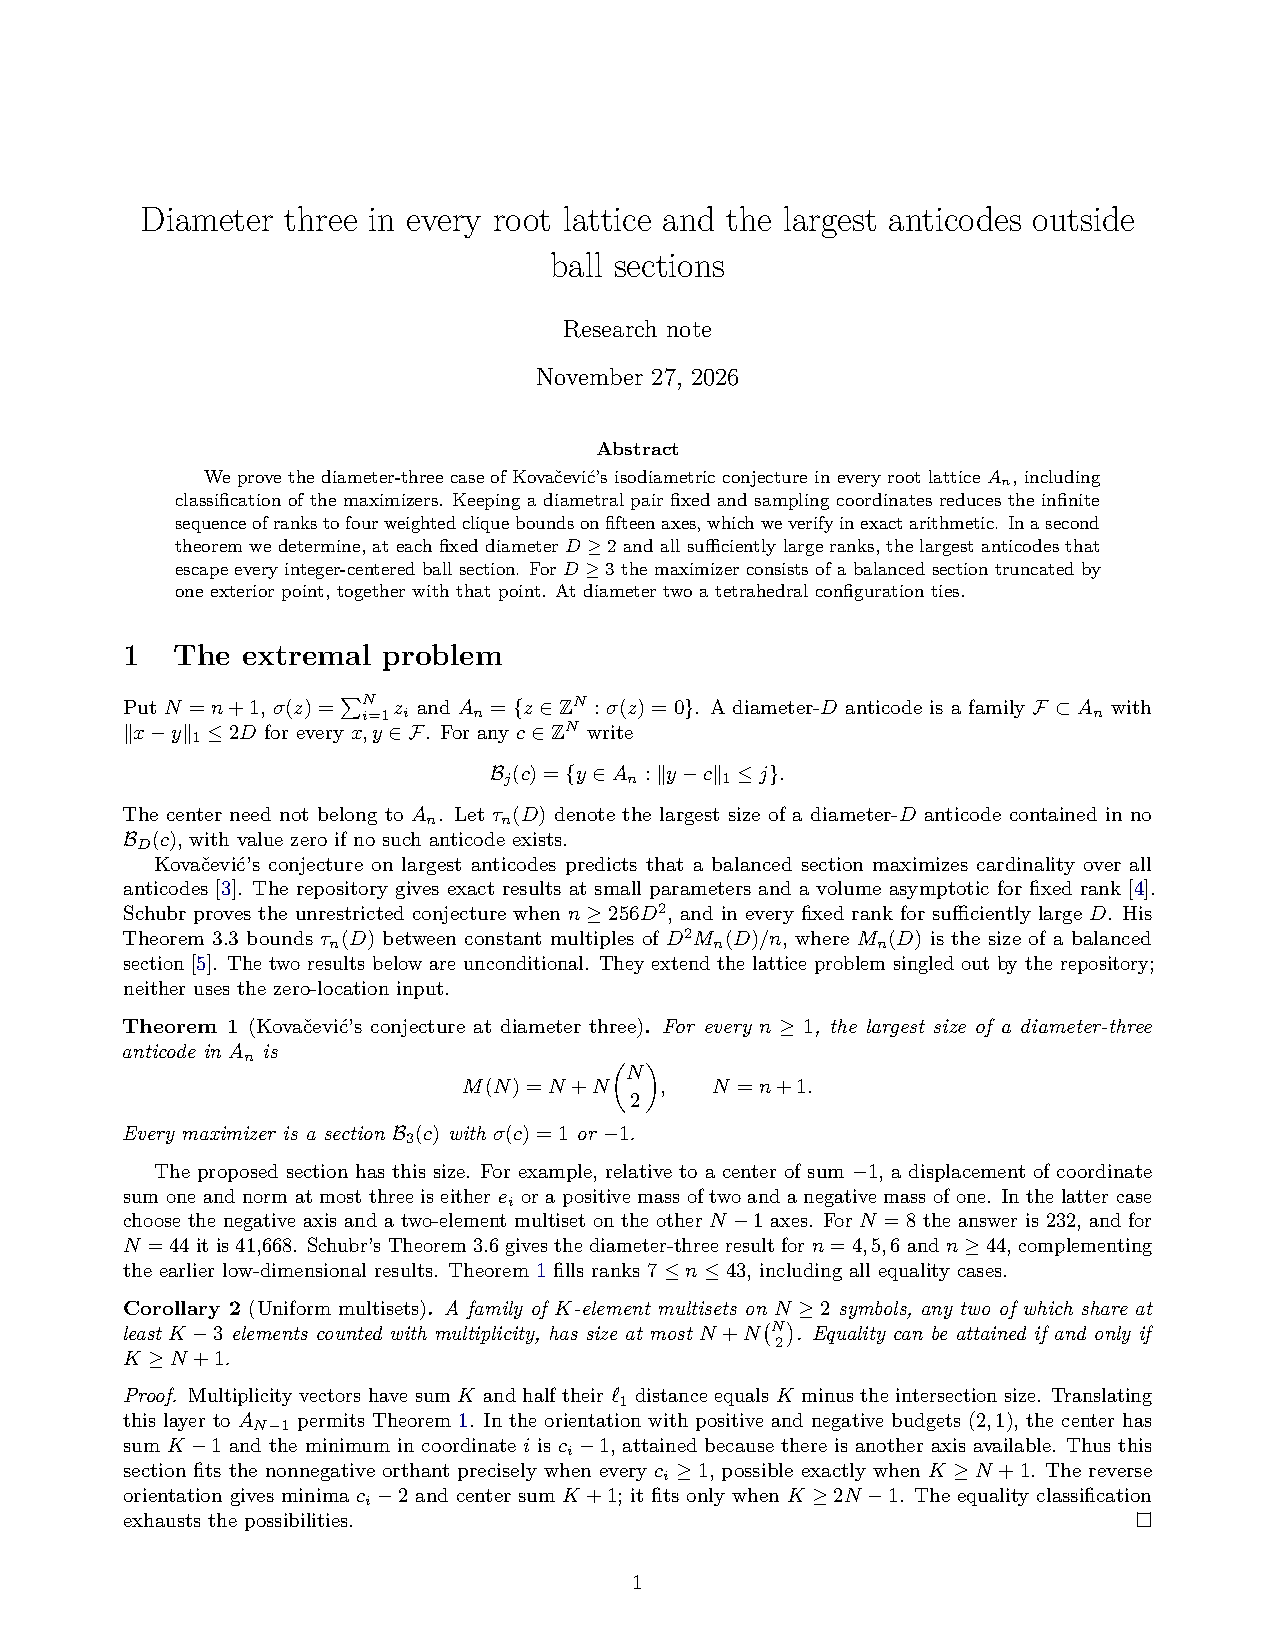
\includepdf[pages=-,addtotoc={1,section,1,Root-lattice anticodes,paperOne}]{anticodes/anticodes.pdf}
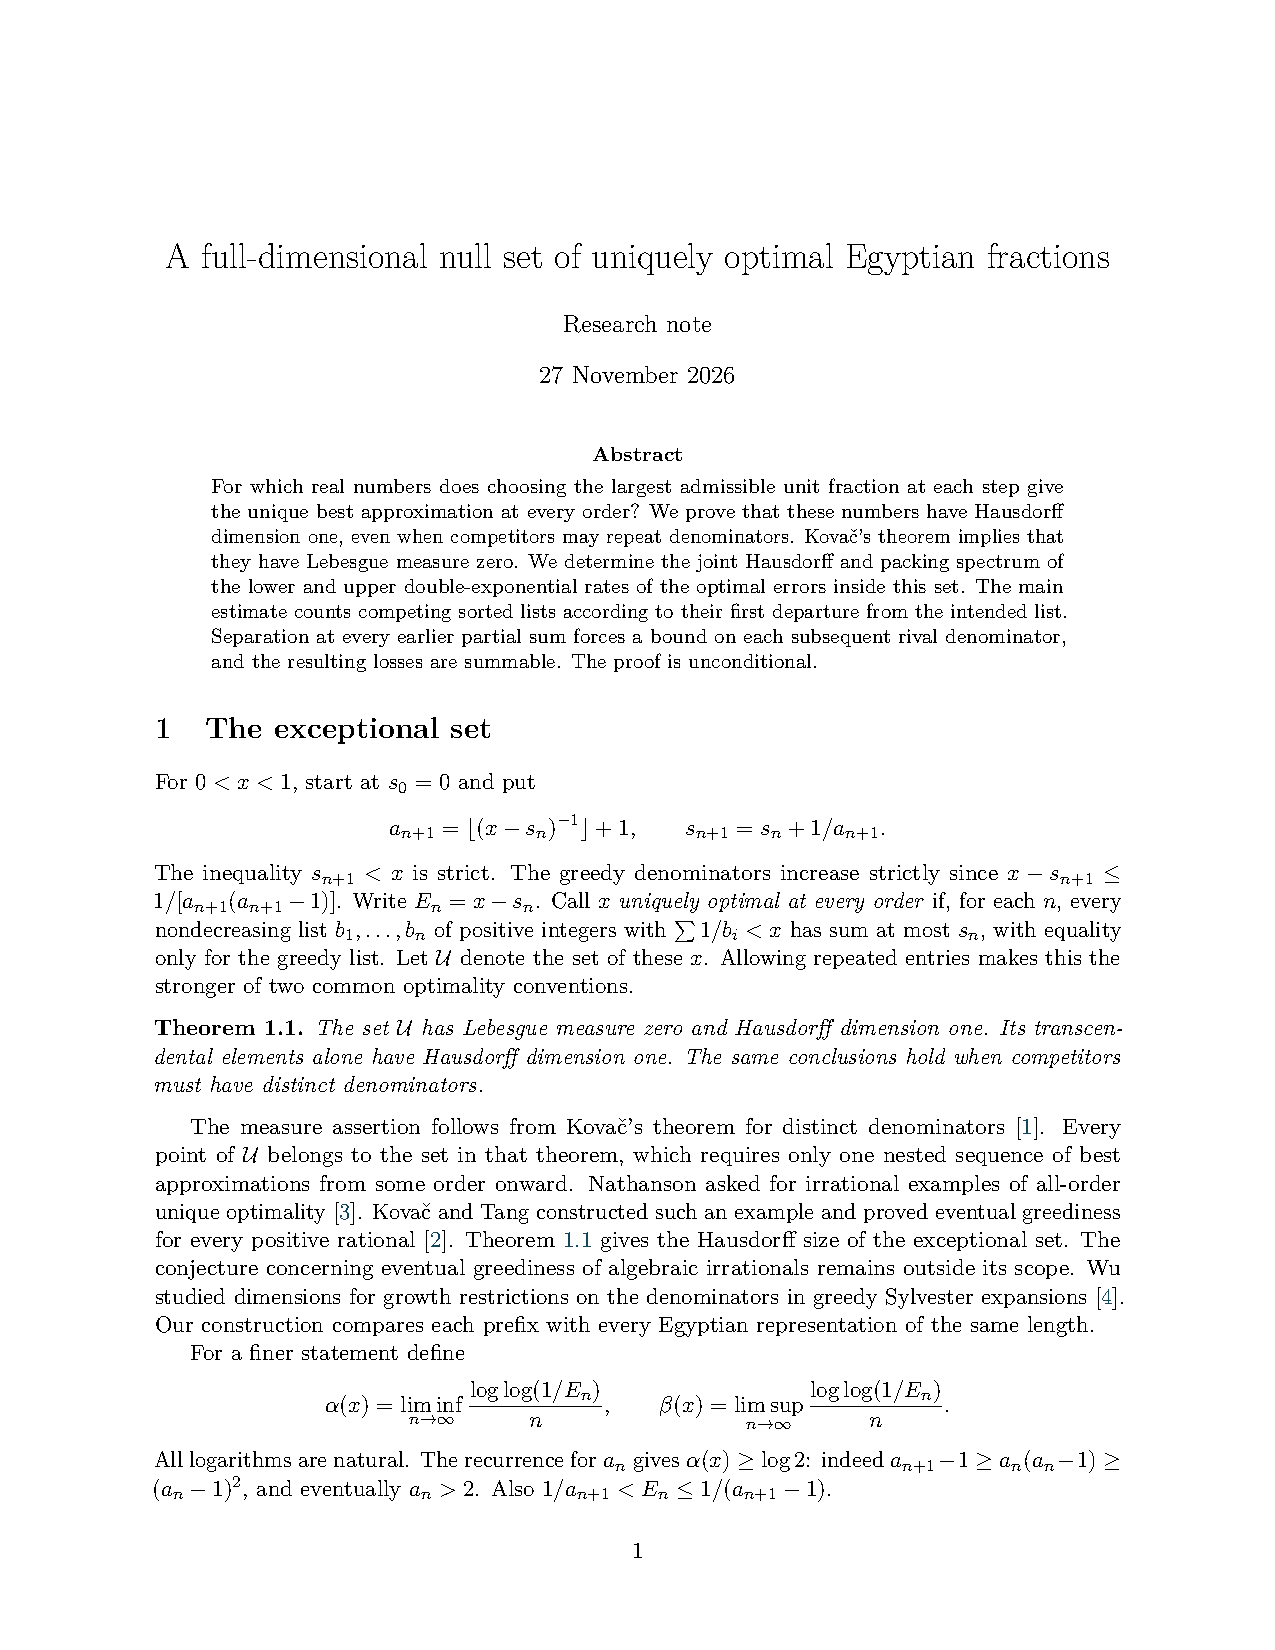
\includepdf[pages=-,addtotoc={1,section,1,Uniquely optimal Egyptian fractions,paperTwo}]{egyptian/greedy-dimension.pdf}
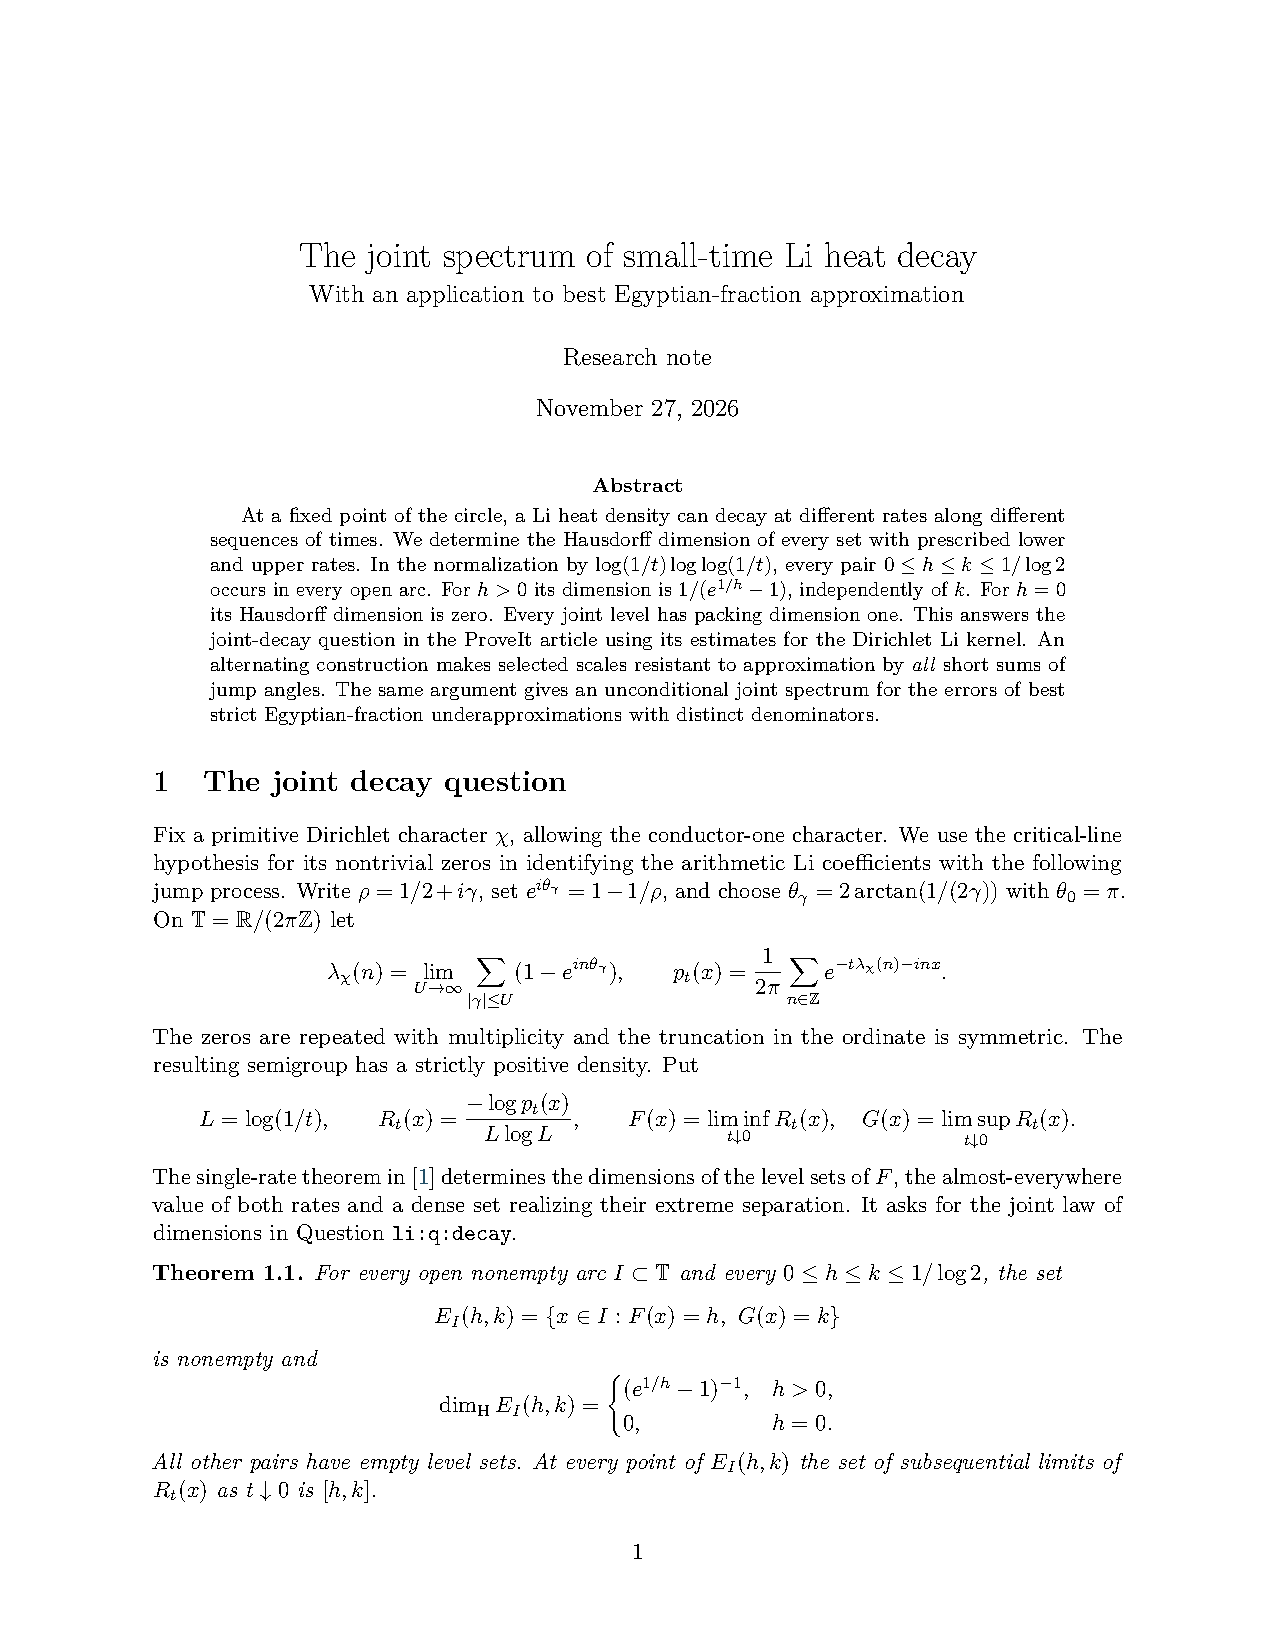
\includepdf[pages=-,addtotoc={1,section,1,Joint decay of Li heat kernels,paperThree}]{li-kernel/joint-spectrum.pdf}
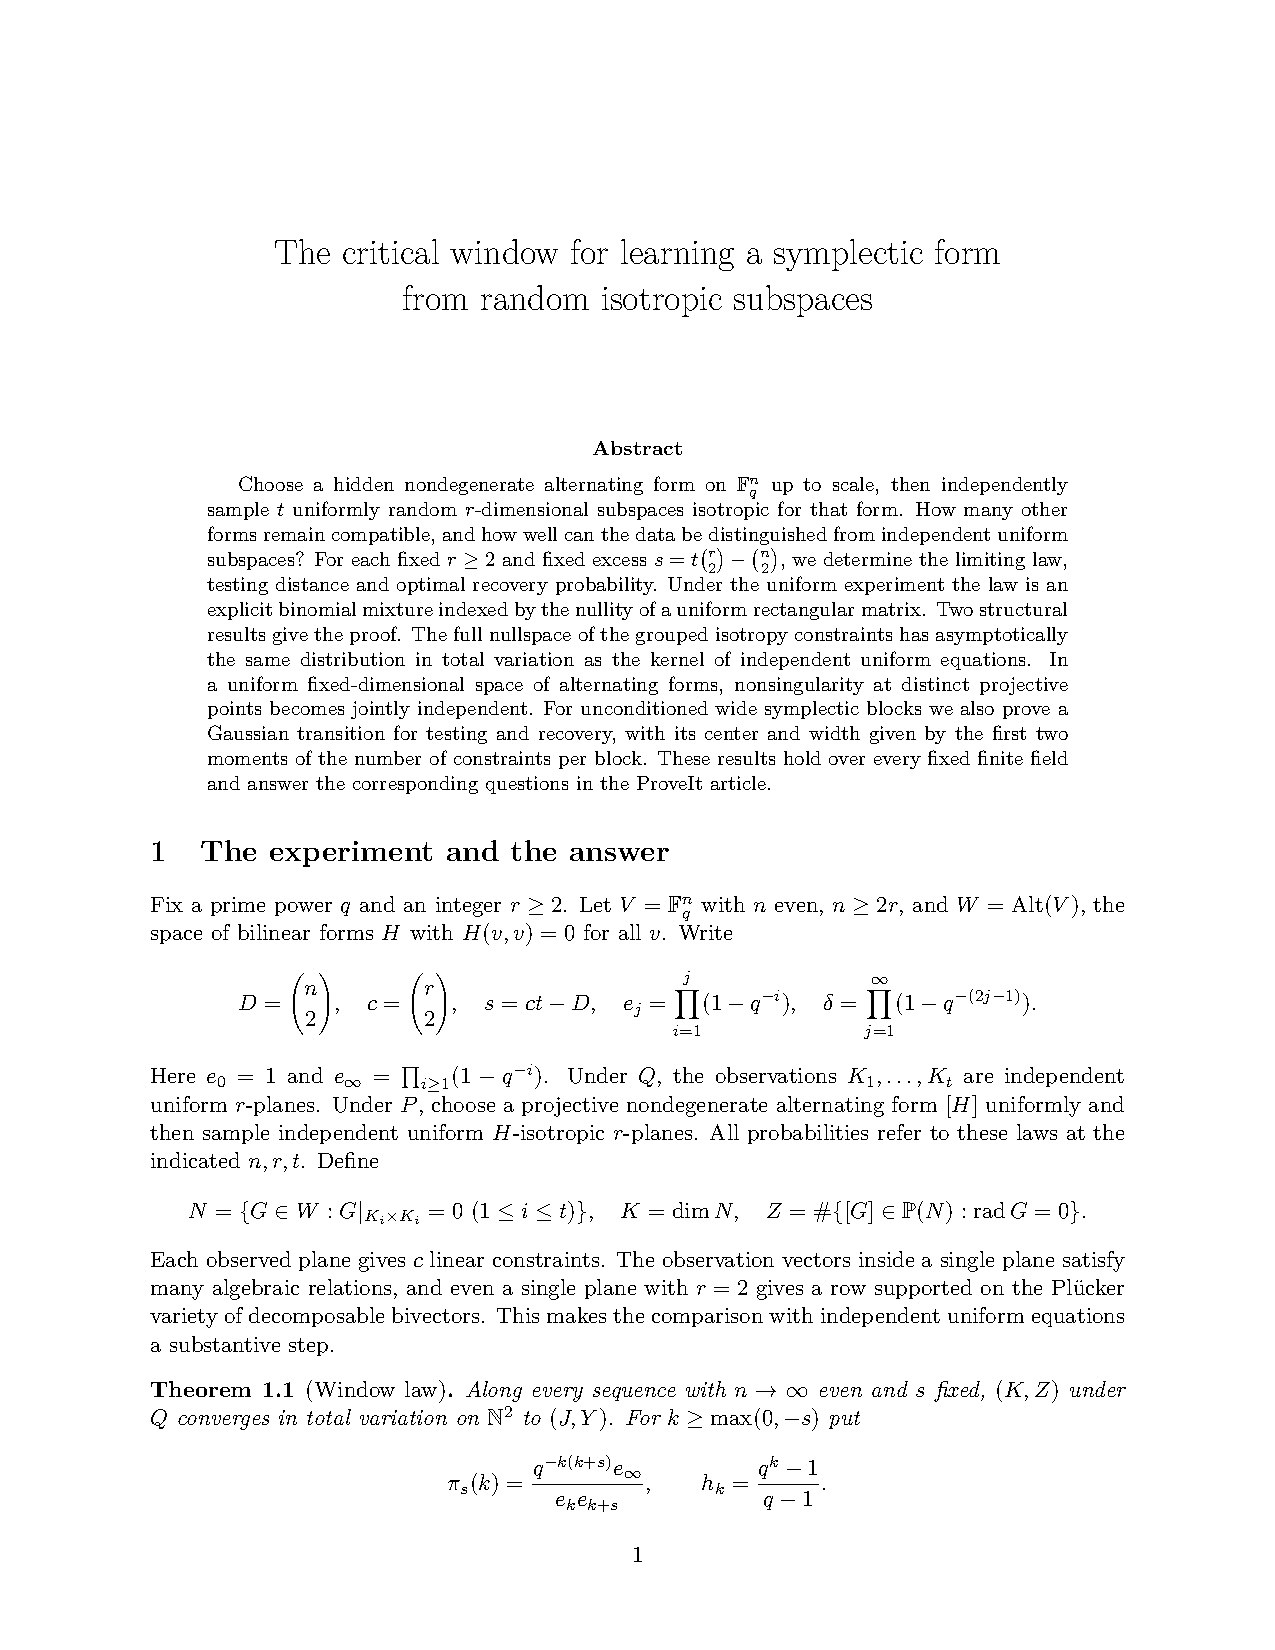
\includepdf[pages=-,addtotoc={1,section,1,Recovery of a symplectic form,paperFour}]{symplectic/hidden_window.pdf}
\end{document}
